\documentclass[a4paper, 11pt, oneside]{report}

%%muy util para salto de línea
%\vspace{0.5 cm}
%Para garantizar la división correcta de palabras en castellano
\usepackage[spanish,activeacute]{babel}
%%\hyphenrules{nohyphenation}

% Conservar division de palabras, listarlas
\hyphenation{} 

\usepackage[pdftex]{graphicx}
%avoid put imagen in specific space
\usepackage{float}
  % declare the path(s) where your graphic files are
  % \graphicspath{{../pdf/}{../jpeg/}}
  \graphicspath{{../imagenes/}}
  % and their extensions so you won't have to specify these with
  % every instance of \includegraphics
\DeclareGraphicsExtensions{.png,.jpeg,}


%Paragraph
%\usepackage{blindtext}

%\usepackage{epsfig}% para los ejemplos con postscript.
%\usepackage{epstopdf}

% inserción url's notas de pie.
\usepackage{url}

%url

\usepackage[colorlinks=true,urlcolor=blue,linkcolor=blue]{hyperref}

%Numeración de página
\setcounter{page}{1}
\pagenumbering{arabic}

%insertat source code
\usepackage{listings}
%%defino atributos para code bash
%%\lstset{language=bash, basicstyle=\ttfamily, frame=single}  \footnotesize
\lstset{basicstyle=\footnotesize\ttfamily, escapechar={', --} }

%comentarios que incluyen varias líneas
\usepackage{verbatim}

%negrita
\usepackage{bold-extra}

% idioma
\usepackage[utf8]{inputenc}
\usepackage[spanish]{babel}

%tablas
\usepackage{booktabs}
\usepackage{multirow}

% Personalizar listas
\usepackage{paralist}

%rotar tablas
\usepackage{rotating}
%formate texto tablas 
\usepackage{array}
%color tablas
\usepackage{colortbl}
%\usepackage[table]{xcolor}
\usepackage{longtable}
%espaciado
\usepackage{setspace}
%%\onehalfspacing
\setlength{\parindent}{0pt}
\setlength{\parskip}{2.0ex plus0.5ex minus0.2ex}

%margenes según n. icontec
\usepackage{vmargin}
\setmarginsrb           { 4.0cm}  % left margin
                        { 3.0cm}  % top margcm
                        { 3.0cm}  % right margcm
                        { 2.0cm}  % bottom margcm
                        {   0pt}  % head height
                        {0.0 cm}  % head sep
                        {   9pt}  % foot height
                        { 1.0cm}  % foot sep

% Paquetes de la AMS:
\usepackage{amsmath, amsthm, amsfonts}
\addto\captionsspanish{\def\refname{\textsc{Bibliografía}}}

\newcommand\portada{
	\begin{titlepage}
		\begin{center}
			{\large \bf ANÁLISIS DE FLUJOS DE INFORMACIÓN EN APLICACIONES ANDROID  \par }
			\vfill
			{\large\bf LINA MARCELA JIMÉNEZ BECERRA \par}
			\vfill
			{\large\bf UNIVERSIDAD DE LOS ANDES  \par}
			{\large\bf FACULTAD DE INGENIERÍA \par}
			{\large\bf DEPARTAMENTO DE INGENIERÍA DE SISTEMAS Y COMPUTACIÓN \par}
			{\large\bf  BOGOTA 2015 \par}
		\end{center}
	\end{titlepage}
}

\newcommand\contraportada{
	\begin{titlepage}
		\begin{center}
			{\large \bf ANÁLISIS DE FLUJOS DE INFORMACIÓN EN APLICACIONES ANDROID \par}
			\vfill
			{\large\bf LINA MARCELA JIMÉNEZ BECERRA \par}
			\vfill
			{\large\bf Asesores\par}
			{\large\bf Martín Ochoa, Ph. D. \par}
			{\large\bf Researcher at the software engineering chair of the TU Munich\par}
			{\large\bf Sandra Julieta Rueda Rodriguez, Ph. D. \par}
			{\large\bf Profesora Asistente, DISC Universidad de los Andes\par}
			\vfill
			{\large\bf UNIVERSIDAD DE LOS ANDES  \par}
			{\large\bf FACULTAD DE INGENIERÍAS \par}
			{\large\bf DEPARTAMENTO DE INGENIERÍA DE SISTEMAS Y COMPUTACIÓN \par}
			{\large\bf BOGOTA 2015 \par}
		\end{center}
	\end{titlepage}
}


\begin{document}

\portada
\contraportada
\tableofcontents
%Modificar el nombre: Índice de cuadros, por Índice de tablas
\renewcommand{\listtablename}{ÍNDICE DE TABLAS}\listoftables
%Modificar el nombre a mayúsculas
\renewcommand{\listfigurename}{ÍNDICE DE GRÁFICAS}\listoffigures
%hacer que el título del capitulo aparezca en mayuscula
\renewcommand\chaptername{CAPÍTULO} 


\label{ch:resumen}
\chapter*{
\begin{center}
	Resumen
\end{center} }
Breve resumen del trabajo : contexo, problema, solución propuesta, resultados
alcanzados.

La presente investigación plantea aplicar técnicas de análisis basadas en
control de flujo de información, con el fin de verificar la ausencia de fugas de
información en aplicaciones Android. Puesto que, controlar el acceso y uso de la
información, representa una de las principales preocupaciones de seguridad en
dichos aplicativos.\newline 
Un estudio reciente de seguridad en dispositivos móviles, publicado por
McAfee\cite{McAfeeReport}, revela que en el contexto de aplicativos Android:
80\% reúnen información de la ubicación, 82\% hacen seguimiento de alguna acción
en el dispositivo, 57\% registran la forma de uso del celular (mediante Wi-Fi o
mediante la red de telefonía), y 36\% conocen información de las cuentas de
usuario.\newline
Diferentes trabajos de investigación han abordado el problema de pérdida de
información en aplicativos Android, sin embargo, la literatura científica
existente al respecto, permite inferir que la mayoría de trabajos aplican
técnicas para hacer data-flow análisis a partir del bytecode. De modo que, su
finalidad es detectar fugas de información y no, verificar que el aplicativo
respeta determinadas políticas de seguridad. Así, el desarrollador de la
aplicación carece de herramientas de apoyo para verificar si la aplicación que
implementa, cumple con determinadas políticas de seguridad.\newline
\label{ch:introduccion}
\chapter{Introducción}
% Información más detallada del contexto en el que se presenta el problema.  
% 
% Datos estadísticos acerca del problema, de los costos que genera, etc.  
% 
% Presentación informal y breve, pero clara, del problema.

En aplicativos Android, el manejo de la información del usuario, es una de las
principales preocupaciones de seguridad. Según un estudio reciente de seguridad
en dispositivos móviles, publicado por McAfee\cite{McAfeeReport}, una importante
cantidad de aplicaciones Android invaden la privacidad del usuario, reuniendo
información detallada de su desplazamiento, acciones en el dispositivo, y su
vida personal.\newline
Por otro lado, para controlar el acceso a información manipulada por sus
aplicaciones, el desarrollador cuenta con los mecanismos de seguridad proveídos por la API de
Android, sin embargo, al estar basados en políticas de control de acceso, se
limitan a verificar el uso de los recursos del sistema acorde a los privilegios
del usuario, lo qué suceda con la información una vez sea accedida, está fuera
del alcance de este tipo de controles. Al no contar con herramientas de análisis
de flujo de información en aplicaciones Android, para el desarrollador es
difícil verificar el cumplimiento de políticas de confidencialidad e integridad
en la aplicación próxima a liberar. Por consiguiente, el desarrollador no tiene como
asegurar la ausencia de fugas de información en la aplicación.\newline
Si bien, en el campo de aplicativos Android, existen diferentes propuestas para
detectar fuga de información, en su mayoría están enfocadas a analizar
aplicaciones de terceros, asumiendo que el atacante provee bytecode malicioso.
Por tanto, aplican data-flow analysis partiendo del bytecode. Estas propuestas
no abordan el problema del lado del desarrollador, analizando flujos de
información de la aplicación para verificar el cumplimiento de políticas de
confidencialidad.\newline
%  hacen falta propuestas que aborden
% el problema análizando flujo de información, 
% mediante técnicas de lenguajes tipados de seguridad(NO ESTOY SEGURA DE ESTA
% AFIRMACIÓN, ES DECIR QUE SÓLO CON SECURITY-TYPED ES POSIBLE DETECTAR FUGAS
% DE INFORMACIÓN),
% lo que se traduce en
% imposibilidad para detección de fugas mediante sentencias de control, por
% ejemplo, la no detección de flujos implicitos.\newline 
Ante esto, y con el fin de proveer una herramienta de apoyo al desarrollador, de
modo que verifique el cumplimiento de políticas de seguridad en sus
aplicaciones, el presente trabajo aborda el problema de fugas de información en
aplicaciones Android, analizando flujos de información de la aplicación,
mediante técnicas de lenguajes tipados de seguridad .\newline


\section{Contexto}
\label{sec:contexto}
%-(Lina: falta actualizar contenido)\newline
Las soluciones propuestas para detectar fuga de información en aplicaciones
Android, se enmarcan en el análisis estático o dinámico de la aplicación, en
algunos casos, se combinan ambos tipos.\newline 
En análisis estático, se estudia el código del programa para inferir todos
los posibles caminos de ejecución. Esto se logra construyendo modelos de estado
del programa, y determinando los estados posibles que puede alcanzar el
programa.
No obstante, debido a que existen múltiples posibilidades de ejecución, se opta
por construir un modelo abstracto de los estados del programa. La consecuencia
de tener un modelo aproximado es pérdida de información y posibilidad de menor
precisión en el análisis.\newline 
Por otro lado, en análisis dinámico se ejecuta el programa y se analiza su
comportamiento, verificando el camino de ejecución que ha tomado el programa.
Esa exactitud en la ejecución que se verifica, da precisión al análisis, porque
no es necesario construir un modelo aproximado de todos los posibles caminos de
ejecución.\newline 
Aunque los resultados del análisis estático pueden perder precisión, la ventaja
es que son generalizables, es decir, el modelo construido representa una
descripción del comportamiento del programa, independientemente de las entradas
y el contexto en que este se ejecute. Ahora, con el análisis dinámico, no es
posible generalizar sus resultados para futuras ejecuciones, porque no
existen garantías de que las entradas para las cuales fue ejecutado el programa,
contengan características para todos los posibles caminos de ejecución.\newline 
Además de las ventajas y desventajas de ambas clases de análisis, cada uno
implica su propio reto, así, mientras en el análisis estático la dificultad está
en construir el modelo de abstracción adecuado, en el análisis dinámico, es
complejo encontrar un conjunto de casos de prueba representativo, a analizar
durante la ejecución del programa.\newline
Por otra parte, dependiendo de la finalidad con qué se detecte la fuga de
información, un tipo de análisis puede ser más apropiado que otro. Si se busca
contener la fuga de información a tiempo de ejecución, análisis dinámico es el
camino apropiado. Por el contrario, si se busca garantizar que a tiempo de
ejecución la aplicación no incurrirá en fugas de información, resulta más
conveniente aplicar análisis estático, porque cumplir con tales garantías
implica definir políticas de confidencialidad y/o integridad desde la
implementación de la aplicación.\newline 
Precisamente, el propósito fundamental del presente trabajo es ofrecer al
desarrollador de aplicaciones Android una herramienta para aplicar políticas de
confidencialidad en la aplicación que implementa, así, la aplicación se
ejecutará exitosamente, si y sólo si, cumple con las políticas definidas, de lo
contrario, el desarrollador puede revisar y corregir su código.\newline
 
En análisis estático, generalmente, se aplican técnicas de seguridad de
tipado(Typed-Inference/Security-Typed Analysis) y técnicas de flujo de
datos(Data/Control Flow Analysis). Con técnicas Security-Typed las propiedades
de confidencialidad e integridad son anotadas en el código, y verificadas a
tiempo de compilación para garantizar que se cumplen en tiempo de ejecución. Con
las técnicas de flujo de control o flujo de datos, se hace seguimiento al flujo
de los datos o control de flujo para verificar el cumplimiento de políticas de
seguridad, generalmente se utilizan grafos de Control de Flujo CFG(Control Flow
Graph), Grafos de Flujo de Datos DFG( Data Flow Graph) y Grafos de llamadas CG
(Call Graphs).\newline 

Al consultar la literatura científica, es posible inferir que parte importante
de las propuestas para análisis de fuga de información en aplicativos
Android(TaintDroid\cite{TaintDroid}, Flow-Droid\cite{FlowDroid-Thesis},
DidFail\cite{DidFail}, DroidForce\cite{DroidForce}), parten del bytecode para
realizar data-flow analysis, mediante técnicas de análisis tainting. Tainting
es un tipo especial de análisis de flujo de datos, que hace seguimiento al flujo
de datos entre un conjunto de fuentes considerados privados y/o sensibles; y un
conjunto de destinos considerados no confiables, sources y sinks,
respectivamente.\newline 
Tales propuestas se enfocan en analizar aplicativos de terceros para detectar
flujos de datos indebidos, y no: para garantizar el cumplimiento de determinadas
políticas de seguridad. En consecuencia, es complejo que el desarrollador
garantice la ausencia de fugas de información en la aplicación que implementa,
partiendo de tales herramientas. Puesto que, al seguir únicamente a los datos
marcados, los datos no marcados para el análisis, pueden acarrear fugas de
información(under-tainting). Adicionalmente, si no se hace seguimiento al flujo
de control pueden existir fugas de información a través de flujos implícitos,
ya que, el análisis estará centrado en flujos explícitos.\newline
No obstante, las limitaciones propias de un análisis basado en flujo de datos,
pueden superarse enfocando el análisis de la aplicación hacia técnicas de
análisis basadas en control de flujo de información, ya que estas analizan el
aplicativo de forma estática para identificar todos los posibles caminos que
podría tomar la aplicación en tiempo de ejecución. Así, con análisis basado en
control de flujo de información, no sólo es posible prevenir fugas por
under-tainting y flujos implícitos; sino que también, es posible ofrecer
garantías del cumplimiento de determinadas políticas de seguridad.\newline 
Ahora, las reglas para evaluar control de flujo de información pueden definirse
mediante técnicas Security-Typed, por ejemplo como se definen con
JIF \ref{JIF-Tool}, una herramienta basada en lenguajes tipados de seguridad
para realizar control de flujo de información, el inconveniente es que está
implementada para aplicaciones en Java, y no para aplicativos Android.\newline 
En general, herramientas como estas, basadas en técnicas de análisis
Security-Typed, implican conceptos como flujo de información, políticas de
confidencialidad e integridad, y chequeo de tipos.\newline 
El flujo de información describe el comportamiento de un programa, desde la
entrada de los datos hasta la salida de los mismos.\newline 
Confidencialidad e integridad son políticas de seguridad, aplicables mediante
control de flujo de información. La confidencialidad busca prevenir que la
información fluya hacia destinos no apropiados, mientras que, la integridad
busca prevenir que la información provenga de fuentes no apropiadas. Una
importante diferencia entre confidencialidad e integridad, es que la integridad
de la información de un programa puede ser alterada sin la interacción con
agentes externos.\newline %\textcolor{red}{(por qué es importante?)}
Ambas políticas son fundamentales para garantizar propiedades de seguridad. Con
políticas de confidencialidad, es posible garantizar ausencia de fugas de
información. Mientras que, con políticas de integridad, la finalidad es evitar
modificación de la información, de forma no consentida.\newline
Por consiguiente, verificar que un programa utilice la información acorde a
tales políticas, implica analizar sus flujos de información, de inicio a fin.
Para el análisis, se deben definir: políticas de flujo de información y
controles de flujo de información, es decir, las políticas de seguridad a
evaluar y los mecanismos para aplicarlas.\newline 
Al usar un lenguaje tipado de seguridad, las políticas son definidas a través
del lenguaje, porque son expresadas mediante anotaciones en el código fuente del
programa a verificar, y su evaluación se realiza mediante chequeo de tipos. El
chequeo de tipos consiste en una técnica estática, también utilizada para
analizar flujo de información durante la compilación de un programa, más
específicamente en la etapa de análisis semántico, el compilador identifica el
tipo para cada expresión del programa y verifica que corresponda al contexto de
la expresión.
%  El
% chequeo de tipos también es una técnica estática utilizada para analizar flujo
% de información durante la compilación de un programa, más específicamente en la
% etapa de análisis semántico, el compilador identifica el tipo para cada
% expresión del programa y verifica que corresponda al contexto de la expresión.
Bajo este principio de chequeo, lenguajes tipados de seguridad aplican
políticas de control de flujo, definiendo para cada expresión del programa un
tipo de seguridad(security type), de la forma:  tipo de dato y label de
seguridad(security label), regulador de uso del dato, acorde a su tipo. El
compilador realiza el chequeo de tipos, partiendo del conjunto de labels de
seguridad. Así, si el programa pasa el chequeo de tipos y compila correctamente,
se espera que cumpla con las políticas de control de flujo evaluadas.

\label{ch:problema}
\chapter{Descripción del problema}

En Android, por defecto, el desarrollador no cuenta con mecanismos para
definir políticas de confidencialidad e integridad que regulen
el flujo de información de sus aplicaciones. Siendo complejo prevenir fugas de
información del usuario, puesto que, el desarrollador carece de herramientas que
le garanticen la ausencia de flujos indeseados.\newline
Precisamente, una de las principales preocupaciones de seguridad en aplicativos
Android, es la manipulación de información del usuario.
Así lo evidencia un
estudio reciente de seguridad en dispositivos móviles, publicado por
McAfee\cite{McAfeeReport}, este señala  que una importante cantidad de
aplicaciones Android invaden la privacidad del usuario, reuniendo información
detallada de su desplazamiento, acciones en el dispositivo, y su vida personal.
De este modo, 80\% reúnen información de la ubicación, 82\%
hacen seguimiento de alguna acción en el dispositivo , 57\%
registran la forma de uso del celular (mediante Wi-Fi o
mediante la red de telefonía), y 36\% conocen información de
las cuentas de usuario.\newline
Las motivaciones para este tipo de acciones varían acorde al tipo de
información, por ejemplo: monitorear información de ubicación para mostrar
publicidad no solicitada; seguir las acciones sobre el dispositivo, para conocer
qué aplicaciones son rentables de desarrollar, o para ayudar a aplicaciones
maliciosas a evadir defensas; acceder a información de cuentas del usuario con
fines delictivos; obtener información de contactos y calendario
del usuario, buscando modificar los datos; obtener información del celular 
(número, estado, registro de MMS y SMS) para interceptar llamadas y enviar
mensajes sin consentimiento del usuario.\newline
Con o sin autorización de acceso, existen motivaciones suficientes para que un
tercero desee manipular información del usuario.\newline
Adicionalmente, el informe señala que una aplicación invasiva no necesariamente
contiene malware, y que su finalidad no siempre implica fraude; de las
aplicaciones que más vulneran la privacidad del usuario, 35\% contienen
malware.\newline 
Si bien, aplicaciones invasivas no necesariamente implican
malware y/o acciones delictivas, el cuestionamiento de fondo es la forma y
finalidad con que están accediendo la información, es decir, si información
de usuario manipulada por una determinada aplicación, realmente debería ser
accedida por otros aplicativos del dispositivo, aún cuando sean considerados no
maliciosos; y qué garantías puede ofrecer el desarrollador para que tal acceso,
efectivamente sea consentido.\newline 
La falta de control sobre los flujos de información de la aplicación puede
ocasionar fugas de información, generando problemas de seguridad tanto para
quien la implementa como para quien la usa.\newline
Como contramedida a este problema, la API de Android ofrece herramientas de
seguridad basadas en políticas de control de acceso, y el desarrollador puede
implementarlas en su aplicación. Sin embargo, estos mecanismos se centran en
regular el acceso de los usuarios del sistema a determinados recursos, y no en
verificar qué sucede con la información una vez es accedida.\newline 
Para superar tal carencia, diferentes trabajos de investigación han abordado el
problema de fuga de información en aplicaciones Android, tanto desde un enfoque
dinámico como desde un enfoque estático, la literatura existente al
respecto(TaintDroid\cite{TaintDroid}, Flow-Droid\cite{FlowDroid-Thesis},
DidFail\cite{DidFail}, DroidForce\cite{DroidForce}), indica que la mayoría de
propuestas hacen data-flow analysis mediante técnicas de análisis usando
tainting, partiendo del bytecode. Una característica sobresaliente entre estos
trabajos es el modelo de ataque, puesto que, se centran en analizar aplicaciones
de terceros asumiendo que el atacante provee bytecode malicioso. Guiar el
análisis de aplicaciones propias con el fin de verificar políticas de
confidencialidad e integridad, bajo tales propuestas, puede implicar: mayor
dificultad en el código a analizar, incompletitud en el análisis(under-tainting)
y no detección de flujos implícitos. Esto debido a que, aún cuando el
desarrollador conoce la funcionalidad de su propio código, las optimizaciones
realizadas por el compilador pueden adicionar complejidad al
mismo\cite[pag.~43]{SecureProgramming}; el seguimiento de los datos a través del
programa está centrado en datos marcados, datos no marcados quedan fuera del
análisis;   flujos de datos a través de estructuras de control, por ejemplo, las
sentencias if, permiten inferir valores de datos marcados como source, sin
necesidad de generar flujos explícitos entre sources y sinks, los cuales si
pueden ser detectados por las técnicas de análisis tainting.\newline Otra razón
fundamental para no  analizar aplicaciones propias con tales propuestas es que
están diseñadas para detectar flujos de datos indebidos, y no para garantizar el
cumplimiento de políticas de seguridad en una aplicación.\newline 
Los riesgos de seguridad tras el under-tainting de datos, y la ausencia de
garantías en el cumplimiento de determinadas políticas de seguridad, pueden
superarse mediante control de flujo de información, Information Flow
Control(IFC), puesto que, con esta técnica se analiza estáticamente la
aplicación para identificar todos los posibles caminos que podrían tomar sus
flujos de información, garantizando que a tiempo de ejecución, la
aplicación respeta políticas de seguridad.\newline

Finalmente, partiendo del contexto que se plantea, dónde se cuenta con el código
fuente Android, porque es el propio desarrollador quien requiere evaluar
políticas de confidencialidad en su aplicación, para  garantizarle
al usuario que la aplicación las cumple. Resulta apropiado proveer una
herramienta de apoyo al desarrollador, mediante la cual analice el flujo de
información de la aplicación próxima a liberar, y verifique el cumplimiento de
políticas de seguridad.
 
\section{Trabajos Relacionados}
\label{sec:trabajo}
\subsection{JIF}
\label{JIF-Tool}
JIF(Java Information Flow), es un lenguaje tipado de seguridad que
permite extender el lenguaje de programación Java,  con control de flujo de
información y control de acceso, usando anotaciones de seguridad. El compilador
usa estás anotaciones durante el chequeo de tipos, verificando el
cumplimiento de la propiedad de seguridad non-interference.

Usar JIF para el análisis estático de flujo de información de un programa,
requiere implementar la versión del mismo, especificando mediante el conjunto de
labels de JIF, las políticas de seguridad a verificar. La implementación de
programas JIF está basada en el modelo de etiquetas DLM(Decentralized Label
Model), donde un principal es una entidad con autoridad para observar y cambiar
aspectos del sistema, así, un principal puede definir y hacer cumplir los
requerimientos de seguridad del dueño de la información. Para expresar una
relación de confianza entre principals, se define la relación acts-for, a partir
de la cual, se derivan dos tipos de principals: top principal y botton
principal, un top principal puede actuar para todos los principals, mientras
que, un botton principal permite que todos los principals actúen para el. Las
políticas de seguridad se condensan en Políticas de Confidencialidad y Políticas
de Integridad, con ellas se determina el conjunto de principals readers y
writes, y el comportamiento que deberían tener.
El compilador de JIF aplica chequeo de labels para verificar  el cumplimiento
de las políticas de seguridad definidas en el programa, cuando determina que
efectivamente las cumple, da paso al compilador de Java para generar su versión
ejecutable.

Además del modelo de labels en que se centra, JIF incluye mecanismos que
aportan características adicionales en la implementación de programas para
seguimiento de Flujo de información. La opción de flexibilizar las políticas
de seguridad de la información, hace parte de estas características adicionales,
y se logra aplicando el mecanismo Downgrading. Dependiendo del tipo política al
que se realiza downgrading, políticas de confidencialidad o políticas de
integridad, el proceso se conoce como Declasificación o Endorsement,
respectivamente.

\subsection{JOANA}
\label{JOANA-Tool}
JOANA (Java Object-sensitive ANAlysis)- Information Flow Control Framework for
Java\cite{JOANA}. Verifica si una aplicación java contiene fugas de
información, mediante análisis estático de flujos de información. El análisis parte  de anotaciones en
el código fuente de la aplicación. JOANA utiliza técnicas de análisis de flujo de
datos y técnicas de análisis de control de flujo. El frontend de la herramienta
está basado en el framework de análisis de programas WALA\cite{wala}, a partir
del cual obtiene la representación intermedia del código Java en forma SSA(Static
Single Assignement), lo que permite obtener información dinámica del programa.
Por otro lado, utiliza Grafos de Dependencia, System Dependence Graphs(SDG),
para detectar dependencias entre las sentencias del programa, es decir,
si existen caminos entre sentencias etiquetadas con nivel de seguridad
alto y sentencias con nivel de seguridad bajo. Para esta etapa del análisis
recurre a técnicas de slicing y chopping, reduciendo la cantidad de caminos
posibles sólo a los válidos. Así obtiene como resultado, una mayor precisión y
reducción de falsas alarmas en el análisis.\newline

Aunque JOANA provee sencillez a la hora de anotar el código a analizar, pues
sólo es necesario anotar inputs y outputs del programa, porque la herramienta se
encarga de propagar las anotaciones en el resto del programa; carece de
características adicionales ofrecidas por sistemas de tipado de seguridad, por
ejemplo, el mecanismo downgrading facilitado por JIF.\newline 

Si bien, al igual que JOANA, la herramienta propuesta a través del presente
trabajo, aplica análisis de control de flujo de información, esta última busca
analizar aplicaciones implementadas en código Android, aprovechando las ventajas
del sistema de anotaciones de JIF. Proporcionando una herramienta de apoyo al
desarrollador de aplicaciones Android, ya que por el momento, JOANA sólo analiza
aplicaciones en JAVA.

\subsection{FlowDroid}
\label{FlowDroid-Tool}
FlowDroid es una herramienta para análisis estático de flujo de datos en
Aplicaciones Android. También permite el análisis de aplicaciones Java.\newline
Esta herramienta utiliza un tipo especial de análisis de flujo de datos:
análisis tainting, que hace seguimiento al flujo de datos entre un conjunto de
sources y un conjunto de sinks. Define tales conjuntos a partir de
SuSi[\ref{sec:susi}], un clasificador automático de sources y sinks para la Api
de Android.\newline 
FlowDroid provee un alto recall y precisión\cite{FlowDroid-Thesis} en el
análisis. El recall, mediante un fiel modelamiento del ciclo de vida de una
aplicación Android; la precisión, incluyendo elementos de análisis como:
context-, flow-, field- y object-sensitive. Para proveer sensibilidad al flujo y
al contexto, recurre a grafos de llamada; y con grafos que modelan todos los
procedimientos del programa(inter-procedural control-flow graph), analiza el
flujo de datos entre procedimientos, proporcionando field- y object-sensitive.\newline
Los autores de esta propuesta, alcanzan precisión en la construcción del grafo
de llamadas extendiendo Soot\cite{Soot}, un framework que genera código
intermedio para código Java y código ejecutable Android(dex). Adicionalmente,
con el framework Heros\cite{heros}, incluyen llamadas multihilos en el análisis
de flujo de datos entre procedimientos.\newline

Entre las limitaciones de FlowDroid está el over-tainting y la no detección
de flujos implícitos. Por tanto, la herramienta no distingue elementos marcados
ni dentro de arrays, ni dentro de collections, si se inserta un elemento marcado
dentro de alguna de estas estructuras, inmediatamente se marca el resto de
elementos. La herramienta tampoco identifica flujos implícitos,    
% causados por dependencias entre control de flujo.\newline
puesto que, según los resultados de evaluación de
DroidBench\cite{DroidBenchBenchmarks}, su benchmark; cuando Flowdroid analiza el
conjunto de aplicaciones de prueba para la identificación de flujos implícitos, no
detecta fuga de datos, generando falsos negativos en la detección de flujos
implícitos\cite[pags 32-36]{FlowDroid-Thesis}.\newline

Aún cuando el problema a atacar es el mismo: fuga de información, la propuesta
que se expone a través del presente trabajo difiere en el enfoque de análisis de
FlowDroid, mientras FlowDroid se concentra en detectar si la aplicación de un
tercero presenta fugas de información, la herramienta planteada aborda el
análisis del lado del desarrollador de la aplicación, apoyándolo en
la verificación del cumplimiento de políticas de seguridad. Así, resulta más
conveniente guiar el análisis mediante control de flujo de información, ya que
se previene fuga por datos no marcados para el análisis(under-tainting) y por
la no detección de flujos implícitos, siendo posible garantizar el cumplimiento
de políticas de seguridad.
 
\subsection{TaintDroid, Dinamic Taint Tracking, para la detección de fugas de
Información}
\label{TaintDroid-Tool}
A diferencia de las propuestas expuestas anteriormente, caracterizadas
por ejecutar el análisis de manera estática, TaintDroid es una herramienta de
análisis dinámico. Está herramienta extiende la plataforma de dispositivos
celulares Android, con el fin de verificar el uso dado por aplicaciones de
terceros a datos sensibles del usuario. El análisis aplica técnicas de análisis
tainting, marcando automáticamente como sources, datos provenientes de fuentes
consideradas privadas y/o sensibles; y como sinks, canales que permiten salir
datos de la aplicación, como por ejemplo internet.
Cada vez que un dato marcado como source sale de la aplicación, se genera un log.\newline 
Para reducir sobrecarga en el dispositivo, pues el análisis es ejecutado a nivel
de instrucciones, instrumentan la máquina virtual de Android con marcas de
propagación a nivel de: variables, métodos, mensajes y archivos. Las marcas de
variable hacen seguimiento a datos dentro de aplicaciones consideras no
confiables. Las marcas de mensaje siguen mensajes entre aplicaciones. Debido a
que TaintDroid no hace seguimiento a la ejecución de código nativo, utiliza las
marcas de métodos para hacer seguimiento a lo retornado luego de invocar métodos
de librerías nativas. Las marcas de archivo son utilizadas para verificar la
persistencia de los datos, acorde a las políticas de seguridad.\newline 
Otra medida para reducir sobrecarga en la ejecución del análisis, consiste en no
hacer seguimiento a flujos de control, generando no detección de flujos
implícitos\cite[pag 12]{TaintDroid}.\newline
Si bien, TaintDroid supera el inconveniente de sobrecarga en la ejecución del
análisis, un inconveniente característico en análisis dinámico, está limitado
para detectar fuga de datos mediante flujos implícitos, puesto que se
enfoca en hacer seguimiento a flujos de datos.\newline 

Al ser una herramienta de análisis dinámico, TaintDroid sólo detecta fugas de
información correspondiente a las ejecuciones presentadas por el programa, y
para la finalidad de su análisis: informar al usuario de posibles fugas de
información, se puede decir que es adecuado. No obstante, para los propósitos de
la propuesta planteada a través del presente trabajo, con la que se pretende
brindar una herramienta de análisis para que el desarrollador verifique el
cumplimiento de políticas de seguridad en la aplicación que implementa, no
resulta viable aplicar análisis dinámico, ni técnicas de análisis tainting para
hacer seguimiento a flujos flujos de datos.
%\subsection{STAMP Análisis estático de aplicaciones}

\subsection{Comparación de técnicas}
Las técnicas utilizadas para análisis de seguridad en aplicaciones, pueden
aplicarse estática o dinámicamente, dependiendo de las propiedades del programa
en que se centre el análisis.\newline
La ejecución dinámica o estática del análisis, trae sus propias ventajas y
desventajas. En el caso de análisis estático, completitud en el análisis es una
de sus principales ventajas. Esto debido a qué, el análisis contempla todas los
caminos de ejecución en que podría incurrir el programa. Evitando que se pierdan
casos a analizar. Por otra parte, al carecer de información que sólo se puede
obtener a tiempo de ejecución, por ejemplo, las entradas que el programa
recibe, el análisis estático suele generar falsos positivos.\newline
En el análisis dinámico, una de las principales ventajas es la baja generación
de falsos positivos, puesto que, el análisis no se centra en los posibles casos
de ejecución, sino que verifica el caso de ejecución que efectivamente está
ocurriendo. No obstante, el análisis dinámico podría incurrir en incompletitud,
porque sólo verifica los casos de ejecución que se presenten, es decir, el
aplicativo podría presentar fugas de información no reportadas por el análisis,
como consecuencia de la no ejecución de los casos que permiten identificarlos.\newline 
Así, el análisis dinámico genera menor cantidad de falsos positivos que el
análisis estático, sin embargo, el análisis estático ofrece mayor completitud en
el análisis.\newline
% Ahora, partiendo del contexto de análisis planteado en el presente trabajo,
% donde el desarrollador cuenta con el código fuente de su propia aplicación y
% pretende garantizar que esta cumple con determinadas políticas de seguridad, la
% característica de completitud en el análisis estático, es cable para garantizar
% el cumplimiento de políticas de seguridad.\newline
Adicional a la forma en que son aplicadas, estática o dinámicamente, las
técnicas de análisis pueden enfocarse en hacer seguimiento al flujo de datos a
través del programa, o en verificar flujos de información. Las técnicas basadas
en tanting análisis, permiten hacer análisis de flujo de datos, marcando los
datos de interés y verificando su flujo entre sources(fuentes del programa
consideradas sensibles y/o confidenciales) y sinks(destinos considerados no
confiables). Entre las desventajas de está técnica, esta el under-tainting, es
decir, la posibilidad de fugas a través de datos no marcados para el
análisis.\newline
Las técnicas para aplicar análisis mediante control de flujo de información,
generalmente permiten definir anotaciones de seguridad en el código fuente de la
aplicación, para verificar sus flujos de información. Estas generalmente se
basan en técnicas de seguridad de tipado(Security-Typed Analyses), o en grafos
que describen el comportamiento del programa, como Contol Dependence Graphs(PDG)
y System Dependence Graphs(SDG).
Ambas técnicas recurren a etapas de análisis de compilación, sin embargo,
mientras las técnicas de Security-Typed sólo requieren llegar hasta el chequeo
de tipos; las basadas en grafos de dependencia deben llegar hasta la
representación de código intermedio para generar los respectivos grafos. Si
bien, con grafos de dependencia se tiene mayor precisión en el análisis, su
ejecución es costosa, ya que genera una complejidad de orden polinomial,
O(N)3\cite[page 3]{FCO-PDG}.
Las motivaciones para guiar el análisis bajo una u otra perspectiva, implica
poner a consideración tanto el nivel de precisión requerido por las propiedades
de seguridad a evaluar, como el costo de implementación y de ejecución del
análisis. \newline


 
%profundizar en las de análisis
% estático, security Typed y control flow \begin{itemize}

% 	  \item El uso de lenguajes de seguridad tipados para el análisis de flujo de
% 	  información en tiempo de ejecución, puede generar sobrecargas.\cite[pag.~1]{LanguageIFS-2013}
% 	  \item Detección de implicit information flows mediante: static enforcements
% 	  of information-flow control versus, run-time enforcement mechanisms.
% 	  \item 
% 	\end{itemize}
% 
% Dentro de las técnicas existentes para adelantar análisis de seguridad en
% aplicativos 
% Para verificar propiedades de seguridad en los aplicativos que implementa, , 
% \begin{itemize}
% 	  \item Information Flow Control
% 	  \item 
% 	  \item 
% 	\end{itemize}
	
\subsection{Clasificación de Sources y Sinks}
\label{sec:susi}
En el ámbito de análisis de flujo de información de aplicaciones,
independientemente del tipo de análisis, estático o dinámico, el punto de
partida es la definición de políticas de privacidad, los pasos sucesivos para 
detectar la perdida de información giran en torno a las políticas de privacidad
definidas.
Muchas de las propuestas para análisis de flujo de información en aplicaciones
Android, parten de un listado de sources y sinks para definir sus políticas de
privacidad. Así, en el grupo de sources se incluyen las fuentes de datos
sensibles, mientras que en el grupo de sinks, se incluyen los medios o canales
que podrían filtrar información sensible de forma no autorizada. 
La efectividad del análisis se ve limitada al listado de sources y sinks, y la
veracidad de los mismos. El inconveniente con estos sources y sinks, es que su
clasificación suele hacerse de forma manual, por tanto, existe mayor
probabilidad de error u omisión.\newline
Con el fin de precisar dicha clasificación, el trabajo de investigación SuSi
propone el uso de machine-learning para la clasificación y categorización de
sources y sinks, partiendo del código fuente de la API Android.
La propuesta de análisis se materializa en una herramienta, que recibe como
entrada métodos de Android y devuelve una lista con la respectiva
categorización de sources y sinks.\newline
La construcción del modelo de
análisis propuesto, parte definiendo los elementos necesarios para el
reconocimiento de sources y sinks; inicialmente define:
Sources y sinks, respectivamente, como las entradas y salidas de flujo de datos del
programa; un dato como un valor o una referencia a un valor; un Resource Method
como un método que lee o escribe datos en un recurso compartido. Seguidamente,
define el concepto de sources y sinks, considerando el contexto de Android:
Android Sources como llamadas a métodos tipo resources(Resources method) que
retornan valores no constantes al código de la aplicación. Android Sinks como
llamadas a methods resource, aceptando como argumento al menos un valor no
constante desde el código de la aplicación, y qué además adicionen o modifiquen
valores del recurso invocado.
El modelo de entrenamiento de SuSi usa el clasificador SMO, una implementación
del clasificador SVM(Support Vector Machines) para Weka, al que inicialmente
enseña a clasificar partiendo de ejemplos entrenados manualmente.
Adicionalmente, lo adapta utilizando la técnica de clasificación
one-againts-all, de modo que pueda representar, tanto los ejemplos de
entrenamiento, en tres clases: sources, sinks, o ninguno; como las
categorías de los sources y sinks identificados.\newline 
Los criterios de clasificación están basados en un conjunto de características,
es decir, funciones que asocian ejemplos de entrenamiento o ejemplos de prueba,
con un determinado valor.\newline
El proceso de análisis se compone de dos rondas secuenciales: clasificación y
categorización. Cada una se compone de las fases input, preparation,
classification y output. Así, la salida de la primera ronda: sources y sinks, se
convierte en entrada para la ronda de categorización, donde se definen
diferentes tipos de categorías, 12 para sources y 15 para sinks.
\section{Background}
\label{sec:back}

\subsection{Aplicaciones Android}
código con ejemplo de componentes(Clases
Activity, ..) 

\subsection{Estructura de trabajo en JIF}
- estructura de los directorios del compilador Jif y estructura de trabajo en
Jif(para entender cómo funciona y cómo afecta el diseño de la
solución).

\subsection{Sintaxis de Anotación en Jif}
\label{subsec:JifSintax}
-Definición de variables: \newline 
\emph{ type\{L\} varName; }\newline 
donde type especifica el tipo de dato que
almacena la variable, \{L\} el label de seguridad  para especificar quien es el
dueño de la variable, y name, el respectivo nombre de la variable.

-Definición de arrays:\newline
en jif un array cuenta con dos labels de seguridad, Base Label(BL) y Size
Label(SL). BL indica el nivel de seguridad de los elementos que almacena el
array, controlando quien puede conocer la información del mismo. SL especifica
quienes pueden conocer la número de elementos almacenados.

-Definición de métodos.\newline
\emph{ type \{RTL\} methodName \{BL\} (arg1\{AL\},,, argn\{AL\}) :\{EL\}
}\newline 
RTL, Return Type Label, indica el label de seguridad con que
queda el tipo de dato devuelto por el método.\newline 
BL begin label, representa el máximo nivel se seguridad del pc label desde donde
se invoca el método, de este modo, el program counter label desde donde
se invoca el método debe ser menor o igual de restrictivo que el BL del
método.\newline 
AL argument label, indica el máximo nivel de seguridad  para los argumentos con
que se llama el método, así, los labels de los argumentos con que se invoca el
método deben ser menor o igual de restrictivos que los AL con que han
definido el método.\newline
EL end label, indica el pc label en el punto de terminación del método, y
representa la información que puede ser conocida.\newline
Cuando un label no es especificado, Jif define unos por defecto. En el caso de
RTL, jif hace un join entre los diferentes AL con que ha sido definido el
método.\newline

\subsection{Métricas de seguridad}
\begin{equation}
\label{p}
	p = TP/(TP +FP) 
\end{equation}
\begin{equation}
\label{r}
	r = TP/(TP+FN) 
\end{equation}

Donde: TP representa el total de verdaderos positivos, FP el
total de falsos positivos y  FN el total de falsos negativos.\newline

\section{Preeliminares para diseño de la solución}
\label{sec:propuesta-sol}
La propuesta para detectar fuga de información en aplicaciones Android, antes de
su publicación, consiste en proveer al desarrollador una herramienta para
análisis estático de flujos de información de la aplicación. Así, partiendo de
las anotaciones de seguridad que el desarrollador defina en el código fuente, se
verifica si la aplicación cumple con políticas de confidencialidad.\newline
Los requerimientos iniciales para construir tal herramienta son: un lenguaje
tipado de seguridad que permita anotar código fuente Android, y el conjunto de
reglas que evaluarán las políticas de confidencialidad.\newline 
Al consultar literatura científica al respecto, se encuentran herramientas como
JIF \ref{JIF-Tool} y JOANA \ref{JOANA-Tool}, especializadas en anotar código
Java, pero no código Android.
Si bien, ambas analizan flujos de información en aplicaciones Java, y podrían
ser extendidas para anotar código Android, las técnicas utilizadas por cada una
son diferentes, por un lado, JIF es un lenguaje tipado de seguridad que basa su
análisis en el chequeo de tipos. Por el otro, JOANA es un framework basado en
análisis de grafos de dependencia. Mientras JOANA se enfoca en precisión, JIF
posee un modelo de anotaciones (DLM) encargado de definir la lattice de
seguridad adecuada para las anotaciones en el código fuente, ofreciendo un
maduro sistema que además de evaluar políticas de confidencialidad, e
integridad, permite definir características de seguridad adicionales como
declasificación y endorsement.
Acorde a los propósitos del presente trabajo, JIF ofrece los beneficios de un
lenguaje tipado de seguridad y un sistema  sólido  de anotaciones, facilitando
la definición de las propiedades de seguridad a verificar.\newline 
Partiendo de JIF como el lenguaje tipado de seguridad, los retos subsiguientes
son: implementar el setup de JIF para Android e integrar a JIF un clasificador
para sources y sinks de Android. El setup de JIF para Android consiste en
implementar las adaptaciones necesarias para que el lenguaje JIF reconozca
código de la API de Android, y admita anotaciones JIF dentro de código
Android, pues aunque en esencia el código Android es código Java, JIF no tiene
como saberlo. También se requiere la integración de un clasificador de sources y
sinks al sistema de anotaciones de JIF, con el fin de proveer información
necesaria para evaluar las políticas de confidencialidad.\newline 
La figura \ref{fig:desing1-in} expone los elementos necesarios para construir la
herramienta de análisis. Básicamente, se requiere un módulo que extienda las
clases en JIF para que el lenguaje reconozca código de la API de Android, es
decir, para que admita anotaciones dentro del código Android: Setup extended JIF
classes. Un módulo que integre el clasificador de sources y sinks de Android al
sistema de anotaciones en JIF:  Android Sources and Sinks. Adicionalmente, se
requiere un modulo que evalúe las políticas de confidencialidad, Checking
Rule Sets, que debe tener comunicación con los módulos anteriormente descritos.
Como entrada, la herramienta recibe el código fuente de la aplicación,
debidamente anotado por el desarrollador, y parte de las anotaciones definidas
para retornar los resultados del análisis.\newline
Habiendo realizado las extensiones necesarias, se espera contar con una
herramienta de análisis de flujo de información, para un conjunto definido de
clases en Android. En la figura \ref{fig:desing1} se ilustra el comportamiento
esperado.\newline

\begin{figure}[t!]
	\begin{center}
	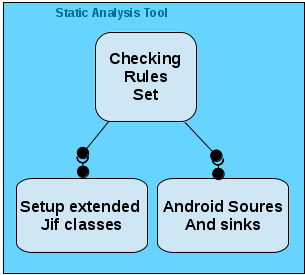
\includegraphics[width=4.6cm]{desing2-inside.png}
	\end{center}
	\caption{Static Analisys Tool Diagrama interno. Ilustra la composición interna
	de la herramienta propuesta para el análisis estático de aplicaciones Android.}
	\label{fig:desing1-in}
\end{figure}

\begin{figure}[t!]
	\begin{center}
	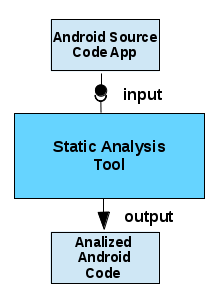
\includegraphics[width=3.5cm]{desing1-2.png}
	\end{center}
	\caption{Static Analisys Tool. Ilustra el input esperado por la herramienta, y
	el resultado devuelto.}
	\label{fig:desing1}
\end{figure} 

Luego, la estrategia de evaluación, consiste en verificar si la herramienta
implementada identifica pérdida de información mediante detección de flujos
implícitos. Esto debido a que, como se menciona en la descripción del problema,
parte importante de las propuestas para detección de fuga de información en
aplicaciones Android, hacen data-flow analysis aplicando técnicas de análisis
tainting, y en contraste con las técnicas de análisis de flujo de información,
las técnicas de análisis tainting no necesariamente consideran flujos
implícitos. Por tanto, al estar basada en JIF, cuyo enfoque de análisis es
precisamente flujo de información, se esperaría que la herramienta planteada
esté en capacidad de reconocer flujos implícitos.

% Se esperaría que: al realizar análisis de flujo de información aplicando
% técnicas Security-Typing, la herramienta propuesta, esté en capacidad de
% reconocer flujos implícitos.\newline
% Más específicamente, se puede tomar el conjunto de aplicaciones utilizadas como
% casos de prueba para la detección de flujos implícitos en
% DroidBench\cite{DroidBenchBenchmarks}, el benchmark de Flowdroid, y analizarlas
% con la herramienta propuesta.\newline

Más específicamente, se puede partir de DroidBench\cite{DroidBenchBenchmarks},
el benchmark de Flowdroid[\ref{FlowDroid-Tool}], tomar el conjunto de
aplicaciones con que prueban la detección de flujos implícitos, y analizarlas
con la herramienta propuesta.\newline
Finalmente estos resultados serían
comparados con los obtenidos mediante otras herramientas para análisis de fuga
de información en aplicaciones Android.\newline

En este orden de ideas, la evaluación de la herramienta propuesta está enfocada
en: medir recall frente a la detección de flujos implícitos, es decir, medir que
no genere falsos negativos ante la existencia de fugas de información,
provenientes de flujos implícitos.\newline

Por último, cabe anotar que aunque la presente propuesta está centrada en
verificar políticas de confidencialidad, en caso de contar con el tiempo
prudente, sería interesante analizar políticas adicionales como por ejemplo,
integridad y declasificación, pues estas son verificables mediante el modelo de
evaluación de JIF, modelo del que parte la herramienta de evaluación planteada.






















\label{ch:desing}
\chapter{Diseño e Implementación}

\section{Limitaciones técnicas para implementar el prototipo}
\label{sec:limitaciones}
Como parte del diseño de la solución, se inicia con una etapa exploratoria. En
esta se anotan manualmente varias aplicaciones de Android, y se identifican
limitaciones del lenguaje Jif para anotar código del framework Android.
Tales limitaciones son adicionales a las características del lenguaje Java no
reconocidas por Jif, a continuación se describen tanto las encontradas, como las
especificadas en el manual de referencia de Jif.

-\textit{Características del lenguaje Java no soportadas por jif}\newline
Si bien, el sistema de anotaciones de Jif hace extensiones al lenguaje java,
permitiendo la evaluación de políticas de confidencialidad e integridad para
aplicativos implementados en dicho lenguaje, el manual de referencia de Jif
precisa las características del lenguaje Java no soportadas\cite{jifRef}. Estas
son:
\begin{itemize}
  \item nested classes: clases que son definidas dentro de otras clases.
  \item initializer blocks: bloques de código declarados dentro de la clase pero
  sin pertenecer a ningún método, dependiendo de si se trata de static
  initialization blocks, su código es el primero en ejecutarse, una vez se
  carga la clase; o si se trata de instance initialization blocks, su código se
  ejecutan cada vez que se crea una instancia de la clase.
\item threads.
\end{itemize} 
Partiendo de estas precisiones, aplicaciones Android que presenten tales
características son excluidas del grupo de aplicaciones a analizar(conjunto de
aplicaciones evaluables) mediante la herramienta propuesta.

% Adicional a las limitaciones de jif frente a características propias del
% lenguaje Java, tras experimentar la anotación manual de una serie de
% aplicaciones Android, se identifican varias limitaciones técnicas para la
% anotación de de las mismas. Entre las limitaciones identificadas están:\newline 

- \textit{Soporte para sobreescritura de métodos}\newline 
En la construcción de aplicaciones Android, según el componente que se esté
implementando(activities, content providers, receivers, services), se requiere
sobreescribir métodos de la clase que extienda el componente. Así, cuando se
define un componente tipo Activity, que debe extender de la clase Activiy.java, 
se sobreescriben métodos como Oncreate. Cada que se sobreescribe
un método se utiliza el statement @Override, con el cual se informa al
compilador de Java que el método es sobreescrito. No obstante, al implementar la
versión Jif de aplicaciones Android con dicho statement, el compilador de Jif
no lo reconoce. La dificultad que se presenta está en el reconocimiento del
statement(carácter @ y clase Override), y no en la sobreescritura de métodos,
puesto que Jif soporta tal característica. El soporte para la sobreescritura de
métodos es confirmado con una sencilla prueba, anotando la clase Activity.java
del framework Android (con un único método, el método Ocreate), e implementando
la versión Jif de una aplicación Android que extiende de tal clase, en la cual
se define una actividad y sobreescribe el método Oncreate.
Cuando se comenta la sentencia @Override, el compilador de Jif identifica la
sobreescritura del método y reporta comentarios para el flujo de información.\newline 
Al investigar el por qué Jif no reconoce tal sentencia, se encuentra que dentro
de las clases Java estándar soportadas por el compilador de Jif, no está
contenida la clase java.lang.Override.\newline
Las clases Java estándar pertenecientes a los paquetes io, lang, math, net y
sql; para las que el compilador Jif brinda soporte, vienen implementadas con
anotaciones en el directorio sig-src, directorio que forma parte de la
distribución del compilador de Jif con que se esté trabajando.\newline
Una alternativa para permitir el análisis de flujo de información entre métodos
que se sobreescriben, es comentar las líneas del programa que contengan la
sentencia @Override, puesto que, al no ser reconocida por el compilador de Jif,
es la generadora de errores de compilación.

- \textit{Casting entre tipos EditText y View}\newline
El framework de Android cuenta con diferentes clases para manejar las interfaces
gráficas que presenta al usuario, entre las cuales se encuentran EditText y
View. View es la clase principal para la creación de widgets, necesarios para la
implementación de componentes interactivos en las interfaces de usuario(UI).
EditText permite adicionar campos de texto editables en UI. El casting entre los
tipos de datos que representan ambas clases, se hace cuando la aplicación debe
procesar datos provenientes de campos en las interfaces del usuario, por ejemplo
como se observa a continuación:
\begin{lstlisting}
EditText editPassword = (EditText)findViewById(R.id.password);
String password = editPassword.getText().toString();
\end{lstlisting}
la interfaz de usuario(que es de tipo View) contiene un campo R.id.password, y
para manipular la información que almacena, debe ser de tipo EditText, siendo
necesario un casting de tipo View a tipo EditText. La dificultad que se presenta
con este tipo de casting es que para el sistema de anotaciones de jif no es
válido. Luego de probar con la anotación manual de ambas clases, tratando de
dar soporte a este tipo de casting, sin obtener resultados satisfactorios, se
opta por ``simular'' estos casos, es decir, si el tipo de dato de una variable
es de tipo EditText, se crea una varible tipo String con un valor determinado,
así se omite el casting y se puede analizar el flujo de información.

- \textit{Clase nested R}\newline
El framework de Android utiliza identificadores para hacer referencia a recursos
utilizados por la aplicación, recursos como strings, widgets y layouts, tales
identificadores son autogenerados en la clase R.java, allí cada recurso es
descrito como una clase individual. Al tratarse de una clase nested, la clase R
no puede ser anotada con jif. Esto puede solucionarse implementando una
versión Jif generalizada de la clase R, que contenga los recursos utilizados en
una aplicación, definidos como variables y no como clases.

- \textit{Sources y Sinks}\newline
En el diseño inicial de la solución se propone utilizar SuSi para clasificar
los sources y sinks en las aplicaciones a analizar, sin embargo, partir del
extenso conjunto de sources y sinks, clasificados por SuSi para la API de
Android, implica una mayor complejidad en el análisis, puesto que, en un
aplicativo todo el código que le conforma puede hacer parte de sources o de
sinks. Adicional a lo complejo que se puede tornar el análisis, los sources y
sinks a considerar deben depender de la política de seguridad a evaluar. En ese
orden de ideas, resulta más viable tomar un subconjunto del listado proveído por
SuSi, partiendo de los sources y sinks que evalué la política de seguridad que
se defina.

- \textit{Enhanced for loop} \newline
Además de soportar la estructura de control for, el lenguaje Java permite el uso
de enhanced for, que es utilizado para simplificar la iteración en arrays y
colecciones, por ejemplo:
% \begin{lstlisting}
% char c[] = imei.toCharArray();
% for (int i = 0; i < c.length; i++) {
% 	obfuscated += c[i] + "_";
% }          
% \end{lstlisting}  
\begin{lstlisting}
for(char c : imei.toCharArray())
obfuscated += c + "_";
\end{lstlisting}
A diferencia de Java, Jif no soporta el enhanced for.\newline
Debido a que ambas sentencias de control son equivalentes, la solución que se
propone para poder analizar flujo de información en los aplicativos Android que
contengan dicha estructura de control, es generar el equivalente del programa
haciendo uso del for, de este modo se cambia la sintaxis sin afectar la lógica
del aplicativo a analizar.

- \textit{Otras limitaciones} \newline
Adicional a las limitaciones descritas anteriormente, para las cuales se propone
una solución, se identifica que Jif no soporta la sintaxis utilizada para
definir estructuras de datos HashMaps, LinkedList y Sets, que en Java se definen
de la siguiente manera:
\begin{lstlisting}
Map<String,String> hashMap = new HashMap<String, String>();
List<String> listData;
Set<String> phoneNumbers = new HashSet<String>();
\end{lstlisting}
Jif tampoco permite la definición de interfaces como argumentos de un método. El
siguiente fragmento de código  en una aplicación Android, muestra la definición
de una interfaz pasada como parámetro al método setOnClickListener.
\begin{lstlisting}
   Button button1= (Button) findViewById(R.id.button1);
   button1.setOnClickListener(new View.OnClickListener() {
   ...
   .....}  });
\end{lstlisting}
En estos casos, la dificultad está en encontrar una sintaxis que permita obtener
la versión equivalente del programa que las contenga. A lo que se suma, la falta
de documentación disponible para solventar los mismos. En consecuencia, se omite
del conjunto de aplicaciones evaluables, aplicaciones Android que requieran en
su implementación las estructuras de datos descritas.\newline

%- \textit{Paso de statements dentro de los argumentos de un método
%(\{\}):}\newline

\section{Diseño de la solución} 
\subsection{Definición de la política de seguridad}
\label{subsection:politica}
Detectar si una aplicación Android(perteneciente al conjunto evaluable) presenta
flujos de información entre, información con nivel de seguridad alto e
información con nivel de seguridad bajo.\newline
Detectando fugas de información catalogada con nivel de seguridad alto, vía:
canales creados durante el control de flujo del programa(flujos implícitos),
mensajes de texto y mensajes de Log.\newline 

\subsection{Consideraciones para verificar el cumplimiento de la política
mediante Jif} 
\label{subsec:consVerPol}
Teniendo definida la política de seguridad a verificar, se describen
elementos influyentes en el diseño de la solución.

\textit{Versión de la API de Android}\newline
Las aplicaciones utilizadas para los experimentos previos a la implementación
del prototipo, y las aplicaciones a anotar con el mismo, se realiza partiendo de
la versión Android 4.2.2(API Level 17).

\textit{Versión del compilador de Jif}\newline
se parte de la versión 3.4.2 del compilador de jif, para llevar a cabo tanto los
experimentos previos como el análisis de las aplicaciones anotadas por el prototipo.

\textit{Diferencia entre una aplicación Android y una aplicación Java
convencional}\newline 
En esencia, una aplicación Android es una aplicación Java con interfaces
descritas en XML, que para ser ejecutada necesita del framework de Android,
porque este le provee acceso al hardware del dispositivo y funcionalidades del
sistema.\newline 
Por otro lado, Jif permite hacer seguimiento al flujo de información de una
aplicación Java, extendiendo el lenguaje mediante labels de seguridad.\newline
Para analizar flujo de información de una aplicación Android mediante
Jif, es importante mencionar que mientras una aplicación Java convencional
cuenta con un único punto de entrada para iniciar su ejecución, esto es, la
clase principal donde se implementa el método main; una aplicación Android puede
tener más de un punto de entrada, generados a partir de los diferentes tipos de
componentes que le integren(Activity, Service, Content Provider y Broadcast
Receiver). La necesidad de interacción del usuario para activar tales puntos de
entrada varía acorde al tipo de componente, así, en el caso de componentes tipo
Activity su ejecución sólo inicia hasta que el usuario interactúe con la
actividad, y para manejar dicha interacción, la API Android provee el método
OnCreate. De otro modo, componentes tipo Service y Broadcast Receiver, inician
su ejecución a través de los métodos OnStartCommand y OnReceive,
respectivamente, sin necesidad de interacción del usuario.\newline 
{ \color{black} {Teniendo en cuenta lo anterior, se asume que la aplicación a
evaluar tiene un único punto de entrada, que depende del tipo de componente que
implemente.} }

\textit{Chequeo de excepciones tipo Runtime}\newline
En lenguaje Java las excepciones tipo Runtime tales como NullPonterException, no
son verificadas a tiempo de compilación, sin embargo, buscando evitar la
generación de canales encubiertos mediante las mismas, Jif si las verifica. 
En consecuencia, si un programa requiere excepciones NullPointerException,
ClassCastException y/o ArrayIndexOutOfBoundsException, el programador debe
declararlas en el programa, de lo contrario, el compilador de Jif genera error.
Para las aplicaciones a analizar, se espera que el desarrollador haya
especificado las excepciones necesarias.

\textit{Información considerada con nivel de seguridad alto}\newline
Para verificar el cumplimiento de la política de seguridad a evaluar se parte de
un conjunto de sources, caracterizados por dar a conocer información del usuario, 
considerada como privada o sensible. Los métodos que integran el conjunto de sources son: 
getDeviceId, getSimSerialNumber, findViewById, getLatitude, getLongitude y
getSubscriberId. Adicional a estos métodos, se incluye el tipo de dato EditText,
si y sólo si, el campo UI al que referencia corresponde a un campo tipo
textPassword, es decir, un campo que almacena contraseñas.

\textit{Canales que muestran información con nivel de seguridad bajo}\newline
La información enviada a través de mensajes de texto y la información conocida
tanto a través de mensajes de Log, como a través de canales generados por el
control de flujo del programa, tiene en común que debe poder ser conocida por
terceros. En consecuencia, se considera que estos canales deben dar a conocer
información con nivel de seguridad bajo.\newline
En el caso de mensajes de texto y mensajes de Log, se hace referencia
específicamente a las clases Log y SmsManager de la API de Android.

\textit{Evaluación del flujo de información}\newline
Para evaluar el flujo de información, se asume que todos los métodos definidos
en la clase serán invocados, y por tanto, todos son incluidos en el análisis.\newline 
Esta decisión de análisis busca evitar el paso inadvertido de flujos de
información, generados por omisión.

\textit{Acceso a métodos de sobreescritura.}\newline
Los métodos de las clases Activity, Service y BroadcastReceiver, son métodos
que se pueden sobreescribir, todo programa Android que extienda de tales clases
debe poder utilizarlos.


\subsection{Pasos para el diseño de la solución}
\label{subsec:pasosSol}
\begin{figure}[t!]
	\begin{center}
	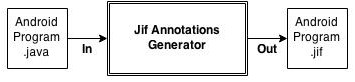
\includegraphics[width=7cm]{desingSolution.jpg}
	\end{center}
	\caption{Entradas y salidas para el generador de anotaciones.}
	\label{fig:desingSolution} 
\end{figure}
Una vez clarificadas las limitaciones técnicas y los elementos a considerar para
el diseño de la solución, se describen los pasos necesarios para la
implementación de la misma. Como se ilustra en la figura
\ref{fig:desingSolution}, la solución a implementar consiste en un anotador de
aplicaciones Android, que recibe como entrada una aplicación
Android(perteneciente al conjunto evaluable), y devuelve la versión Jif del
mismo, el cual contiene las anotaciones para evaluar la política de seguridad
definida.\newline

\textit{Paso uno: hacer que Jif reconozca determinadas clases de la API de
Android}.

\begin{figure}[h!]
	\begin{center}
	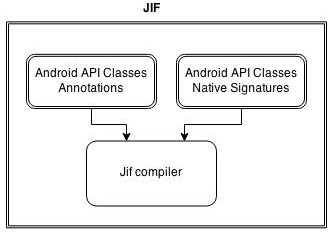
\includegraphics[width=5cm]{desingSol-steps1.jpg}
	\end{center}
	\caption{Tipos de anotación necesarias para implementar la solución.}
	\label{fig:desingSol-steps1}
\end{figure}

\begin{figure}[t!]
	\begin{center}
	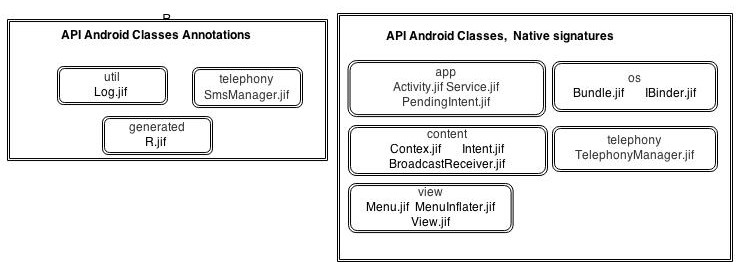
\includegraphics[width=12cm]{desingSol-step1-details.jpg}
	\end{center}
	\caption{Diseño de la solución paso 1. Ilustra las clases especificas de la
	API de Android, anotadas manualmente.}
	\label{fig:desingSol-details}
\end{figure}
Adicional al mecanismo de anotación que se maneja en Jif, en que para hacer
análisis al flujo de información de un programa Java, se debe implementar la
versión del respectivo programa para Jif. También es posible adicionar clases
Java ya existentes, utilizando signaturas nativas para que el compilador Jif las
reconozca, esto es: generando una versión Jif de la clase java, donde se
declaran constructores y cuerpo de los métodos a utilizar de la clase fuente
Java.\newline
Para el presente trabajo se utilizan ambas opciones de anotación. Tal como se
ilustra en la figura \ref{fig:desingSol-steps1}. 
El criterio para decidir que se anota de una u otra forma, depende de lo que
represente la clase Android para verificar la política de seguridad establecida.
Las clases Log y SmsManager, que representan canales para conocer información,
son anotadas de forma no nativa. La opción de anotación nativa se utiliza para
librerías Android, por ejemplo la clase TelephonyManager necesaria para utilizar
el método getDeviceId. En la figura \ref{fig:desingSol-details} se especifican
clases de la API Android a anotar.\newline

\textit{Paso dos: Definir Autoridades y forma de anotación del programa Android
a analizar.}\newline
Una clase Android tendrá una Autoridad máxima(un principal), en este caso Alice,
así que, información con nivel de seguridad alto deberá pertenecer a dicha
autoridad.\newline
Jif hace seguimiento al flujo de información del programa, asociando un label
de seguridad al program counter de cada sentencia y expresión del programa,
program counter(pc) label. Este pc es afectado por el label de seguridad que se
especifique en la declaración de variables y métodos\ref{subsec:JifSintax}. 
Partiendo de que Jif se fundamenta en labels de seguridad para hacer seguimiento
al flujo de información del programa, es necesario definir los labels a
anotar para métodos y variables del programa.\newline
En el caso de variables con nivel de seguridad  alto, la anotación debe
ser:\newline
\emph{ type\{Alice:\} varName; }\newline
Para el resto de variables, entran a jugar las anotaciones definidas por Jif
acorde al contexto donde están definidas.\newline
Ahora en el caso de los métodos, la anotación varía según si el método debe
influenciar(acceder, modificar) o no, información anotada con nivel de seguridad
alto.

En base a lo anterior, se define un algoritmo de anotación que se condensa en un
generador de anotaciones; y se fundamentado en las siguientes
definiciones:\newline \textit{Definición A:} anotación de variables con nivel de
seguridad alto:\newline modifier type\{Alice:\} varName;\newline 
\textit{Definición B:} métodos que se sobreescriben. El sistema de anotaciones
de Jif exige que el nivel de seguridad del método desde donde se invoca la
sobreescritura de un método, no debe ser menos restrictivo que el método a
sobreescribir, y los métodos a sobreescribir deben poder ser invocados desde
todo programa Android, siguiendo con este principio, y buscando que jif no
limite el flujo de información, estos métodos deben ser anotados con BL
público(\{\}).\newline 
\textit{Definición C:} anotación de métodos con sources\newline
Los labels para la definición del método(BL, EL, AL )se anotan de la
siguiente manera:\newline modifier type
nameMethod\textit{\{Alice:\}} type\textit{\{Alice:\}}
( arg1,.....type\textit{\{Alice:\}}argn ) \{\}\newline Si dentro del método se
definen arrays, sus respectivos BL y SL, deben ser anotados así: modifier type\{Alice:\}[ ]\{Alice:\}\newline
\textit{Definición D:} anotación de métodos que no reciben información del
source. 
nameMethod\textit{\{\}}(
type\textit{\{Alice:\}}arg1,.....type\textit{\{Alice:\}}argn ) \{\}\newline
Teniendo claras las anteriores definiciones, los pasos para el algoritmo son los
siguiente:\newline
(1) Identificar sources de la clase. Si se encuentran sources continuar con
los pasos (2) a (4), sino, continuar con paso (2) y aplicar definiciones B y
D.\newline
(2) Identificar el total de métodos de la clase.\newline
(3) Del total de métodos listar los que son invocados con el source.\newline
(4) Del total de métodos listar los que no son invocados con el source.\newline
(5) Aplicar definición C a listado del paso(3).\newline
(6) Aplicar definición D a listado del paso (4).\newline
(7) Aplicar definición B. \newline
(8) Aplicar definición A a listado del paso (1).

\subsection{Descripción implementación prototipo}
-Diagrama de clases o descripción


%\label{ch:implementacion}
\chapter{Implementación}

Detalles de implementación \newline

Usuarios y atacantes habilitados para observar la ejecución de un programa,
debe ser el marco de partida para la definicón de políticas de seguridad e
integridad, de la información de un programa.\newline

Teniendo claras las políticas, se requiere un análisis exaustivo del
programa, verificando que efectivamente estén siendo aplicadas.\newline

El resultado del análisis debería mostrar que la información controlada por
tales políticas, no fluye hacia ambitos del progrma que violen las respectivas
reglas.\newline
  
\label{ch:evaluacion}
\chapter{Evaluación}
Ventajas y limitaciones de la solución.\newline 
Si aplica, evaluación de desempeño.  \newline 
Si aplica, evaluación de usabilidad.  
Hay otras soluciones similares? \newline 
Cuáles son las diferencias y las ventajas y desventajas con respecto a esas soluciones.

\section{Consideraciones de evaluación}
No se consideran flujos de información vía interAppComunicación. Por ejemplo,
varias aplicaciones que se comunican entre sí.

\section{Evaluación conjunto de aplicaciones}
Para la evaluación del prototipo se toma un grupo de testcases de DroidBech, el
benchmark de FlowDroid, aplicables para la evaluación de la política de
seguridad establecida.\newline 
Se considera con nivel de seguridad alto, variables y métodos que almacenan y
modifican(respectivamente), información considereada como privada(Sources).\newline 
Se considera con nivel de seguridad bajo, canales para envío de mensajes,
muestra de logs y canales creados durante el flujo del programa.\newline
A continuación se describen los testcases a evaluar, en los casos en que se
requiere, se precisan observaciones entre los resultados de evaluación esperados
para la técnica de análisis utilizada por FlowDroid y la técnica de análisis
propuesta en el presente trabajo.\newline
% \textbf{AndroidSpecific\_DirectLeak1}\newline
% La variable \textit{mrg} tiene un nivel de seguridad alto, almacena
% información retornada por el método source \textit{getDeviceId}. Se genera
% flujo de información directo entre información con nivel de seguridad alto e
% información con nivel de seguridad bajo, al enviar como parámetro del método
% \textit{\textbf{sendTextMessage}}, información de la variable \textit{\textbf{mrg}}.

\begin{table}[H]
\small\addtolength{\tabcolsep}{-3pt}
\caption{Descripción aplicaciones de prueba}
\label{tb:descripApps}
\begin{tabular}{|p{13cm}|p{1cm}|}
	\hline
	\multicolumn{2}{|>{\columncolor[gray]{0.8}}c|}{\textbf{AndroidSpecific\_DirectLeak1}}\\
	\hline
	\textbf{Descripción} & \textbf{Leaks}\\
	\hline
	La variable \textit{mrg} tiene un nivel de seguridad alto,
	almacena información retornada por el método source \textit{getDeviceId}. Se
	genera flujo de información directo entre información con nivel de seguridad alto e
	información con nivel de seguridad bajo, al enviar como parámetro del método
	\textit{sendTextMessage}, información de la variable \textit{mrg}. & 1 \\
	\hline
	\multicolumn{2}{|>{\columncolor[gray]{0.8}}c|}{\textbf{AndroidSpecific\_InactiveActivity}}\\
	\hline
	\textbf{Descripción} & \textbf{Leaks}\\
	\hline 
	La variable \textit{imei} tiene un nivel de seguridad alto, almacena
	información retornada por el source getDeviceId. La variable es enviada como
	parametro a \textit{Log}, canal que muestra información con nivel de
	seguridad bajo. \textit{Observación:} debido a que la actividad en que se
	presenta este flujo de información no está activada en el Manifest de la
	aplicación, para la técnica de análisis de FlowDroid no existen leaks. Para
	nuestra propuesta de análisis si existe leak, porque se asume que los métodos y
	sus aplicaciones podrán ser ejecutados. & 0
	\\
	\hline
	\multicolumn{2}{|>{\columncolor[gray]{0.8}}c|}{\textbf{AndroidSpecific\_LogNoLeak}}\\
	\hline
	\textbf{Descripción} & \textbf{Leaks}\\
	\hline
	El caso de prueba no presenta información con niveles de seguridad alto. Se
	presentan flujos de información entre información con el mismo nivel de
	seguridad, en este caso bajo, lo cual es permitido. & 0 \\
	\hline
	\multicolumn{2}{|>{\columncolor[gray]{0.8}}c|}{\textbf{AndroidSpecific\_Obfuscation1}}\\
	\hline
	\textbf{Descripción} & \textbf{Leaks}\\
	\hline 
	La variable \textit{\textbf{mrg}} tiene un nivel de seguridad alto,
	almacena información retornada por el método source getDeviceId().
	Se genera flujo de información entre información con nivel de seguridad alto e
	información con nivel de seguridad bajo, al enviar como parámetro del método
	\textit{sendTextMessage}, información de la variable
	\textit{mrg}. \textit{Observación:} el elemento adicional para este
	testcase es proveer una suplantación de la clase
	android.telephony.TelephonyManager, en el apk de la aplicación. Para la
	evaluación que proponemos, se verifica acorde a la versión que se tiene anotada
	para esta clase, es decir, independientemente de la obfuscación de la clase,
	nuestro análisis debe detectar que existe un flujo de información indebido. &
	1\\
	\hline
	\multicolumn{2}{|>{\columncolor[gray]{0.8}}c|}{\textbf{AndroidSpecific\_PrivateDataLeak2}}\\
	\hline
	\textbf{Descripción} & \textbf{Leaks}\\
	\hline
	La variable \textit{info} tiene un nivel de seguridad alto, almacena
	información suministrada por el campo EditText de tipo textPassword. Se genera
	flujo de información entre información con nivel de seguridad alto e
	información con nivel de seguridad bajo, al pasar la variable
	\textit{info} como parámetro de \textit{Log}, que muestra
	información con nivel de seguridad bajo. & 1 
	\\
	\hline
	\multicolumn{2}{|>{\columncolor[gray]{0.8}}c|}{\textbf{ArraysAndLists\_ArrayAccess1}}\\
	\hline
	\textbf{Descripción} & \textbf{Leaks}\\
	\hline
	Se tiene un array en que se almacena información tanto proveniente como no
	proveniente de sources, parte de la información que almacena es envíada como
	parámetro del método \textit{sendTextMessage}. \textit{Observación:}
	Para la técnica de análisis de FlowDroid(tainting), se marca únicamente el
	indice del array donde se almacena el dato considerado como source, así,
	cuando se envía como parámetro del método \textit{sendTextMessage},
	el dato de un indice no marcado, no se genera leak. Para nuestra técnica
	de análisis(flujo de información mediante JIF), para que un array almacene
	información con nivel de seguridad alto, primero debe ser catalogo(anotado)
	con nivel de seguridad alto, lo que implica que el array podrá almacenar
	información tanto de nivel de seguridad alto como bajo, pero toda la
	información quedará con nivel de seguridad alto. En consecuencia, al enviar
	cualquier indice del array como parámetro del metódo 
	\textit{sendTextMessage} se presenta un flujo de información no
	permitido. & 0
	\\
	\hline
\end{tabular}
\end{table}

\begin{table}[H]
\small\addtolength{\tabcolsep}{-3pt}
\caption{Descripción aplicaciones de prueba}
\label{tb:descripApps}
\begin{tabular}{|p{13cm}|p{1cm}|}
	\hline
	\multicolumn{2}{|>{\columncolor[gray]{0.8}}c|}{\textbf{ArraysAndLists\_ArrayAccess2}}\\
	\hline
	\textbf{Descripción} & \textbf{Leaks}\\
	\hline
	Se presenta el contexto descrito en ArraysAndLists\_ArrayAccess1, con un
	elemento adicional, se implementa el método calculateIndex(), que calcula el
	indice del array a ser envíado como parámetro del método
	\textit{sendTextMessage}. & 0 \\
	\hline
	\multicolumn{2}{|>{\columncolor[gray]{0.8}}c|}{\textbf{GeneralJava\_Exceptions1}}\\
	\hline
	\textbf{Descripción} & \textbf{Leaks}\\
	\hline
	La variable \textit{imei} es de nivel de seguridad alto, almacena información
	devuelta por el método \textit{getDeviceId}. Se genera flujo de información
	entre información de nivel de seguridad alto e información con nivel de
	seguridad bajo, al enviar como parametro del método \textit{sendTextMessage}
	información de la variable \textit{imei}. Este flujo de información se presenta
	dentro de la captura de una excepción RuntimeException(no es verificada
	en tiempo de compilación).
	& 1
	\\
	\hline
	\multicolumn{2}{|>{\columncolor[gray]{0.8}}c|}{\textbf{GeneralJava\_Exceptions2}}\\
	\hline
	\textbf{Descripción} & \textbf{Leaks}\\
	\hline
	La variable \textit{imei} es de nivel de seguridad alto, almacena información
	devuelta por el método \textit{getDeviceId}. El control de flujo del
	programa conduce de manera implícita a la captura de una excepción tipo
	RuntimeException, desde allí se utiliza información proveida por la variable
	\textit{imei}, como parámetro para invocar el método \textit{sendTextMessage}.
	Generando un flujo de información indebido. & 1
	\\
	\hline
	\multicolumn{2}{|>{\columncolor[gray]{0.8}}c|}{\textbf{GeneralJava\_Exceptions3}}\\
	\hline
	\textbf{Descripción} & \textbf{Leaks}\\
	\hline
	La variable \textit{imei} es de nivel de seguridad alto, almacena información
	devuelta por el método \textit{getDeviceId}. La información proveida por
	\textit{imei} es utilizada como parámetro para invocar el método
	\textit{sendTextMessage} dentro de la captura de una excepción tipo
	RuntimeException, sin embargo, el programa no genera un caso que haga ejecutar
	la captura de la excepción. & 0
	\\
	\hline
	\multicolumn{2}{|>{\columncolor[gray]{0.8}}c|}{\textbf{GeneralJava\_Exceptions4}}\\
	\hline
	\textbf{Descripción} & \textbf{Leaks}\\
	\hline
	La variable \textit{imei} es de nivel de seguridad alto, almacena información
	devuelta por el método \textit{getDeviceId}. información proveída por esta
	variable es envíada como parámetro para la captura de una excepción en tiempo
	de ejecucón, donde es utilizado como parámetro para invocar el método
	\textit{sendTextMessage}, generando un flujo de información indebido. & 1\\
	\hline
	\multicolumn{2}{|>{\columncolor[gray]{0.8}}c|}{\textbf{GeneralJava\_Loop1}}\\
	\hline
	\textbf{Descripción} & \textbf{Leaks}\\
	\hline
	La variable \textit{imei} es de nivel de seguridad alto, almacena información
	devuelta por el método \textit{getDeviceId}. Se generan flujos de información
	indebidos, primero al tratar de asignar la información de la varianle a un
	array con nivel de seguridad bajo(donde se intenta ofuscar la información),
	luego al tratar de enviar la información ofuscada como paramétro del método
	\textit{sendTextMessage}, con nivel de seguridad bajo. & 1 \\
	\hline
	\multicolumn{2}{|>{\columncolor[gray]{0.8}}c|}{\textbf{GeneralJava\_Loop2}}\\
	\hline
	\textbf{Descripción} & \textbf{Leaks}\\
	\hline
	La variable \textit{imei} es de nivel de seguridad alto, almacena información
	devuelta por el método \textit{getDeviceId}. Se busca ofuscar la información de
	\textit{imei} mediante ciclos for anidados, allí se asigna la información de la
	varianle a un array con nivel de seguridad bajo. Luego se envía la información
	ofuscada, como parámetro del método \textit{sendTextMessage}, con nivel de
	seguridad bajo, gerendo otro flujo de información indebido. & 1\\
	\hline
\end{tabular}
\end{table}

\begin{table}[H]
\small\addtolength{\tabcolsep}{-3pt}
\caption{Descripción aplicaciones de prueba}
\label{tb:descripApps}
\begin{tabular}{|p{13cm}|p{1cm}|}
	\multicolumn{2}{|>{\columncolor[gray]{0.8}}c|}{\textbf{GeneralJava\_UnreachableCode}}\\
	\hline
	\textbf{Descripción} & \textbf{Leaks}\\
	\hline
	La variable \textit{deviceid} con nivel de seguridad alto, está contenida en un
	método que no es llamado, dentro del mismo, \textit{deviceid} es pasada como
	parámetro para invocar el método \textit{sendTextMessage}, cuyo nivel de
	seguridad es bajo. \textit{Observaciones:} para el análisis de FlowDroid el
	programa no presenta leaks, ya que el método nunca es llamado.
	Para nuestro análisis, el programa presenta leak porque se asume que todos los
	métodos son llamados. & 0\\
	\hline
	\multicolumn{2}{|>{\columncolor[gray]{0.8}}c|}{\textbf{ImplicitFlows\_ImplicitFlow1}}\\
	\hline
	\textbf{Descripción} & \textbf{Leaks}\\
	\hline
	 La variable \textit{imei} con nivel de seguridad alto, almacena información
	 devuelta por el método \textit{getDeviceId}, \textit{imei} se pasa como
	 parámetro al método obfuscateIMEI que devuelve la información ofuscada.
	 Después se invoca el método WriteToLog, con la información ofuscada como
	 parámetro para ser mostrada en el log. Al invocar el método WriteToLog con la
	 información ofuscada, se genera un flujo de información indebido. & 1 \\
	\hline
	\multicolumn{2}{|>{\columncolor[gray]{0.8}}c|}{\textbf{ImplicitFlows\_ImplicitFlow2}}\\
	\hline
	\textbf{Descripción} & \textbf{Leaks}\\
	\hline
	 La variable \textit{userInputPassword} con nivel de segurida alto, almacena
	 información de un campo EditText tipo textPassword(password suministrado por
	 el usuario). Se generan flujos de información indebidos: al tratar de asignar
	 información a la variable passwordCorrect con nivel de seguridad bajo, a
	 partir de la comparación de información con nivel de seguridad alto(variable
	 textPassword), después, al tratar de mostrar en el \textit{log} información
	 que depende de tal comparación. & 1\\
	\hline
	\multicolumn{2}{|>{\columncolor[gray]{0.8}}c|}{\textbf{ImplicitFlows\_ImplicitFlow4}}\\
	\hline
	\textbf{Descripción} & \textbf{Leaks}\\
	\hline
	La variable \textit{password} con nivel de seguridad alto, almacena información
	de un campo EditText tipo textPassword, \textit{password} es utilizada como
	parte de los parámetros para invocar el método \textit{lookup} que busca
	identificar el password sumisnitrado por el usuario. Se genera un flujo de
	información indebido, cuando se compara lo retornado por el método para mostrar
	en el \textit{log} información del password. & 1 \\
	\hline
	\multicolumn{2}{|>{\columncolor[gray]{0.8}}c|}{\textbf{Lifecycle\_ActivityLifecycle3}}\\
	\hline
	\textbf{Descripción} & \textbf{Leaks}\\
	\hline
	 El flujo de información entre información con nivel de seguridad alto e
	 información con nivel de seguridad bajo, tiene lugar a través de dos
	 métodos del ciclo de vida de la actividad: onSaveInstanceState y
	 onRestoreInstanceState. En onSaveInstanceState, se asigna información con
	 nivel de seguridad alto a la variable \textit{s}, la información que almacene
	 este método es utilizada durante la reanudación de la actividad, a través del
	 método onRestoreInstanceState, donde se muestra en el \textit{log} información
	 de la variable \textit{s}. & 1\\
	\hline
	\multicolumn{2}{|>{\columncolor[gray]{0.8}}c|}{\textbf{Lifecycle\_BroadcastReceiverLifecycle1}}\\
	\hline
	\textbf{Descripción} & \textbf{Leaks}\\
	\hline
	 Se tiene un broadcast receiver  que muestra información con nivel de
	 seguridad alto, contenida en la variable \textit{imei}(almacena información retornada por el
	 método \textit{getDeviceId}) a través del \textit{log}. & 1 \\
	\hline
	\multicolumn{2}{|>{\columncolor[gray]{0.8}}c|}{\textbf{Lifecycle\_ServiceLifecycle1}}\\
	\hline
	\textbf{Descripción} & \textbf{Leaks}\\
	\hline
	 Se tiene un servicio que presenta flujo de información indebida mediante dos
	 métos de su ciclo de vida. En el método que inicia el servicio
	 onStartCommand, la variable con nivel de seguridad alto, almacena
	 información devuelta por el método \textit{getDeviceId}. Luego el método
	 onLowMemory, se envía información de la variable \textit{secret} a través de
	 un mensaje msm. & 1\\
	\hline
\end{tabular}
\end{table}

La tabla\ref{tb:comparacion} presenta los resultados de analizar los casos de
prueba previamente descritos, tanto con FlowDroid como con el prototipo. Los
resultados se califican como: Falso Positivo(FP) cuando se detecta un leak que
no existe; Falso Negativo(FN) cuando no se detecta un leak existente; Verdadero
Positivo(TP) cuando se detecta un leak existente; Verdadero Negativo(TN) cuando
no existe leak que detectar.\newline 
Se utiliza el comando \textit{time} para medir el tiempo requerido para
realizar el análisis.
 
\begin{table}[H]
\small\addtolength{\tabcolsep}{-3pt}
\caption{Comparación Precisión entre FlowDroid y Prototipo}
\label{tb:comparacion}
\begin{tabular}{|p{5.8cm}|p{1cm}|p{2.1cm}|p{2.1cm}|p{1cm}|p{1cm}|}
	\hline
	\textbf{Testcase} & \textbf{Leaks} & \textbf{FlowDroid} &
	\textbf{Prototipo} & \textbf{ t F} & 
	\textbf{t P}\\
	\hline
	AndroidSpecific\_DirectLeak1 & 1 & TP & TP &5.371s &2.063s\\
	\hline
	AndroidSpecific\_InactiveActivity & 0 & TN & FP  &3.255s &2.469s\\
	\hline
	AndroidSpecific\_LogNoLeak & 0 & TN & TN &5.505s &2.946s\\
	\hline
	AndroidSpecific\_Obfuscation1 & 1 & TP & TP &6.734s &2.706s\\
	\hline
	 AndroidSpecific\_PrivateDataLeak2 & 1 & TP & TP & 6.144s &2.644s\\
	\hline
	 ArraysAndLists\_ArrayAccess1 & 0 & FP & FP & 4.708s & 1.278s\\
	\hline
	 ArraysAndLists\_ArrayAccess2 & 0 & FP & FP & 4.4s &1.361s\\
	 \hline
	 GeneralJava\_Exceptions1 & 1 & TP & TP &6.397s &2.755s\\
	\hline
	 GeneralJava\_Exceptions2 & 1 & TP & TP &5.887s &1.980s\\
	\hline
	GeneralJava\_Exceptions3 & 0 & FP & FP &6.008s &2.032s\\
	\hline
	GeneralJava\_Exceptions4 & 1 & TP & TP &5.731s &2.313s\\
	\hline
	GeneralJava\_Loop1 & 1 & TP & TP &5.605s &2.800s\\
	\hline
	GeneralJava\_Loop2 & 1 & TP & TP &4.719s &1.361s\\
	\hline
	GeneralJava\_UnreachableCode & 0 & TP & FP &3.792s &1.197s\\
	\hline
	ImplicitFlows\_ImplicitFlow1 & 1 & FN & TP &4.853s &1.331s\\
	\hline
	ImplicitFlows\_ImplicitFlow2 & 1 & FN & TP &4.496s &1.212s\\
	\hline
	ImplicitFlows\_ImplicitFlow4 & 1 & FN & TP &4.375s &1.224s\\
	\hline
	Lifecycle\_ActivityLifecycle3 & 1 & TP & TP &4.792s &1.222s\\
	\hline
	Lifecycle\_BroadcastReceiverLifecycle1 & 1 & TP & TP &4.456s &1.061s\\
	\hline
	Lifecycle\_ServiceLifecycle1 & 1 & TP & TP &5.225s &1.180s\\
	\hline
\end{tabular}
\end{table}

-\textit{Resultados de precisión}\newline
En lo que respecta a los resultados del Prototipo, los FP correspondientes a
AndroidSpecific\_InactiveActivity y GeneralJava\_UnreachableCode, surgen como
consecuencia de realizar el análisis asumiendo que el desarrollador utiliza lo
que implementa.\newline 
Por otro lado, en el caso de ArraysAndLists\_ArrayAccess1 y
ArraysAndLists\_ArrayAccess2, no es sencillo calificar los resultados como FP,
puesto que, para lo que está analizando FlowDroid(verificar que su técnica de
análisis diferencie entre los elementos marcados y no marcados de un array),
efectivamente se presentan FP, sin embargo, para la forma en que se deben
implementar los programas en jif, donde se suele definir un nivel de seguridad
para todo el array antes de almacenar los elementos en el mismo, podría decirse
que no se trata de un FP, porque se revelo información que había sido
catalogada.\newline 
La detección de flujos implícitos podría ser un elemento diferenciador.\newline
-\textit{Resultados de desempeño}\newline
Se podría destacar como positivo que el análisis de flujo de información
mediante técnicas de tipado de seguridad, requiere menos tiempo que la técnica
de marcado de datos utilizada por FlowDroid.


\label{ch:trabajoFuturo}
\chapter{Trabajo Futuro y Conclusiones}
\section{Discusión}
Límites de la solución propuesta 

\section{Trabajo Futuro}
Cómo puede ser extendido el trabajo y qué beneficios tendría esa extensión 

\section{Conclusiones}
Qué aprendimos con este trabajo.  
\bibliographystyle{IEEEtran}
\bibliography{referencias}
\end{document}